\begin{boxK}
% در زبان ++C یا Python یک پیام را با الگوریتم AES ،رمزگذاری یا رمزگشایی کنید.

یک پیام را با الگوریتم
\grayBox{\lr{AES}}
در زبان
\grayBox{\lr{Python}}
یا
\grayBox{\lr{C++}}
رمزگذاری یا رمزگشایی کنید.
\end{boxK}

\begin{boxL}
برای این منظور پیام 
\grayBox{\lr{Shahid Ghasem Soleimani}}
را در نظر گرفته‌ایم.

با استفاده از کتابخانه
\grayBox{\lr{pycryptodome}}
عملیات رمزگذاری را انجام داده‌ایم.

یک کلید ۱۶ بیتی را ایجاد خواهیم کرد. سپس رشته بیتی رمزشده را
(\grayBox{\lr{Cipher Text}})
در فایل
\grayBox{\lr{encrypted.bin}}
ذخیره‌سازی خواهیم کرد.

در سلول بعدی عملیات رمزگشایی را انجام خواهیم داد.
\end{boxL}

\begin{figure}[h]
    \centering
    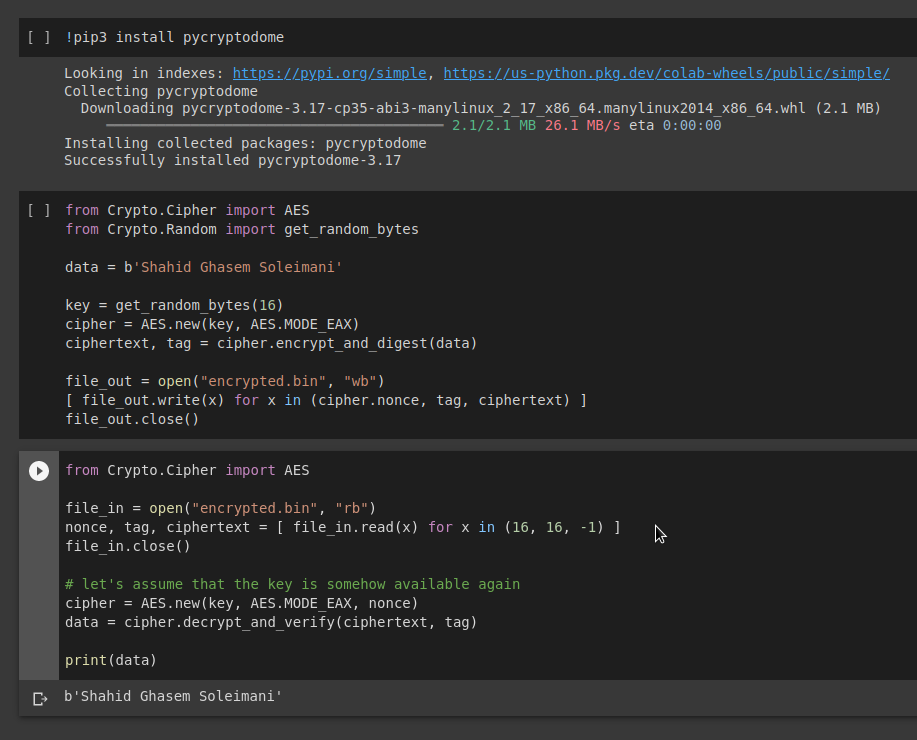
\includegraphics
    [width = 0.8\textwidth]
    {HW3/images/aes_1.png}
    \caption{تصویری از اجرای این الگوریتم}
    \label{fig:my_label}
\end{figure}

